\documentclass[spec, och, labwork]{shiza}
% параметр - тип обучения - одно из значений:
%    spec     - специальность
%    bachelor - бакалавриат (по умолчанию)
%    master   - магистратура
% параметр - форма обучения - одно из значений:
%    och   - очное (по умолчанию)
%    zaoch - заочное
% параметр - тип работы - одно из значений:
%    referat    - реферат
%    coursework - курсовая работа (по умолчанию)
%    diploma    - дипломная работа
%    pract      - отчет по практике
% параметр - включение шрифта
%    times    - включение шрифта Times New Roman (если установлен)
%               по умолчанию выключен
\usepackage{subfigure}
\usepackage{tikz,pgfplots}
\pgfplotsset{compat=1.5}
\usepackage{float}

%\usepackage{titlesec}
\setcounter{secnumdepth}{4}
%\titleformat{\paragraph}
%{\normalfont\normalsize}{\theparagraph}{1em}{}
%\titlespacing*{\paragraph}
%{35.5pt}{3.25ex plus 1ex minus .2ex}{1.5ex plus .2ex}

\titleformat{\paragraph}[block]
{\hspace{1.25cm}\normalfont}
{\theparagraph}{1ex}{}
\titlespacing{\paragraph}
{0cm}{2ex plus 1ex minus .2ex}{.4ex plus.2ex}

% --------------------------------------------------------------------------%


\usepackage[T2A]{fontenc}
\usepackage[utf8]{inputenc}
\usepackage{graphicx}
\graphicspath{ {./images/} }
\usepackage{tempora}

\usepackage[sort,compress]{cite}
\usepackage{amsmath}
\usepackage{amssymb}
\usepackage{amsthm}
\usepackage{fancyvrb}
\usepackage{listings}
\usepackage{listingsutf8}
\usepackage{longtable}
\usepackage{array}
\usepackage[english,russian]{babel}

% \usepackage[colorlinks=true]{hyperref}
\usepackage{url}

\usepackage{underscore}
\usepackage{setspace}
\usepackage{indentfirst} 
\usepackage{mathtools}
\usepackage{amsfonts}
\usepackage{enumitem}
\usepackage{tikz}
\usepackage{minted}

\newcommand{\eqdef}{\stackrel {\rm def}{=}}
\newcommand{\specialcell}[2][c]{%
\begin{tabular}[#1]{@{}c@{}}#2\end{tabular}}

\renewcommand\theFancyVerbLine{\small\arabic{FancyVerbLine}}

\newtheorem{lem}{Лемма}

\begin{document}

% Кафедра (в родительном падеже)
\chair{}

% Тема работы
\title{Алгоритм шейкерной сортировки}

% Курс
\course{3}

% Группа
\group{331}

% Факультет (в родительном падеже) (по умолчанию "факультета КНиИТ")
\department{факультета КНиИТ}

% Специальность/направление код - наименование
%\napravlenie{09.03.04 "--- Программная инженерия}
%\napravlenie{010500 "--- Математическое обеспечение и администрирование информационных систем}
%\napravlenie{230100 "--- Информатика и вычислительная техника}
%\napravlenie{231000 "--- Программная инженерия}
\napravlenie{100501 "--- Компьютерная безопасность}

% Для студентки. Для работы студента следующая команда не нужна.
% \studenttitle{Студентки}

% Фамилия, имя, отчество в родительном падеже
\author{Окунькова Сергея Викторовича}

% Заведующий кафедрой
% \chtitle{} % степень, звание
% \chname{}

%Научный руководитель (для реферата преподаватель проверяющий работу)
\satitle{доцент} %должность, степень, звание
\saname{А. Н. Гамова}

% Руководитель практики от организации (только для практики,
% для остальных типов работ не используется)
% \patitle{к.ф.-м.н.}
% \paname{С.~В.~Миронов}

% Семестр (только для практики, для остальных
% типов работ не используется)
%\term{8}

% Наименование практики (только для практики, для остальных
% типов работ не используется)
%\practtype{преддипломная}

% Продолжительность практики (количество недель) (только для практики,
% для остальных типов работ не используется)
%\duration{4}

% Даты начала и окончания практики (только для практики, для остальных
% типов работ не используется)
%\practStart{30.04.2019}
%\practFinish{27.05.2019}

% Год выполнения отчета
\date{2022}

\maketitle

% Включение нумерации рисунков, формул и таблиц по разделам
% (по умолчанию - нумерация сквозная)
% (допускается оба вида нумерации)
% \secNumbering

%-------------------------------------------------------------------------------------------
\tableofcontents

\section{Описание алгоритма}

Шейкерная сортировка (Cocktail sort), она же сортировка перемешиванием, она же двунаправленная 
сортировка — по сути всего лишь оптимизированный алгоритм пузырьковой сортировки, в основе котрой
также лежит сравнение двух соседних элементов. Единственное отличие состоит лишь в том, что теперь 
это происходит в двух направлениях поочередно, постепенно сужая диапазон сортировки. В итоге за один 
проход в конец массива “всплывает” максимальный элемент из диапазона, а за следующий проход — в начало 
массива минимальный. Эти элементы можно больше не рассматривать и таким образом диапазон сужается с 
двух сторон.
\section{Эффективность алгоритма}

Сложность работы алгоритма в худшем случае определяется как $O(n^2)$, так как суммарное количество 
сравнений равно $(n - 1)\frac{n}{2}$, а число обменов равно $(n-1)\frac{n}{2}$, где n - это размер
входного массива, что делает эту сортировку не самой эффективной в классе сортировок.

Сложность работы алгоритма в лучшем случае определяется как $O(n)$, так как суммарное количество 
сравнений равно $(n - 1)\frac{n}{2}$, а число обменов равно $0$, где n - это размер входного массива.
Этот случай достигается тогда, когда на вход подается уже отсортированный массив.

Главным плюсом данной сортировки является то, что она не требует выделения дополнительной памяти.

\section{Реализация}

    \inputminted[fontsize=\small]{cpp}{lab1.cpp}

\section{Тестирование программы}

\begin{figure}[H]
    \centering      %размер рисунка       здесь находится название файла рисунка, без указания формата
    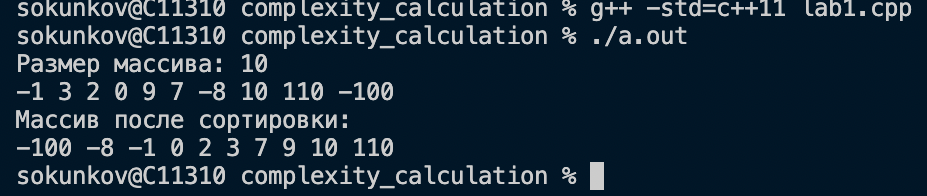
\includegraphics[width=1.\textwidth]{1}
    \caption{Тест1}
    \label{fig:image1}
\end{figure}

\newpage

\begin{thebibliography}{3}
    \bibitem{1}
    Скиена Стивен "Алгоритмы. Руководство по разработке", 2018 год. Яз. рус.
    \bibitem{2}
    Нииколаус Вирт "Алгоритмы и структуры данных", 2008 год. Яз. рус.
\end{thebibliography}

\end{document}